\section{Network}
Devices that are exchanging data are connected with each other and form a network. The ability of a device to connect one to another is provided by the network interface of a device. 

The network interface can use the \gls{ip}. Before a client can send data it needs to know about the presence and how to address the other device. Each device has a unique address inside the network which is called IP-Address. The IP-Address can be assigned either by a \gls{isp}, a \gls{dhcp} Server or it can have a static one in a local environment. 
Data is transmitted in form of IP-Packets. The IP-Packet has the IP-Address of the sender and of the receiver and next to other fields the actual payload \cite{roberts}.

To transfer an IP-Packet from one device to another a router is needed which connects two networks and is forwarding packets either inside the local network or to the other connected network as described by \cite{shuler2002}.
Each device is registering itself at the router. The router then stores the IP-Address in a routing table. All devices known by the router are representing the local network. 

When the router receives an IP-Packet it looks up the receiver IP-Address in its routing table and is then forwarding the packet to the receiver when an entry exists.
When no entry exists the packet is forwarded to another network. The router of the other network is taking care of it. The other router is repeating the process until some router knows the receiver.
To prevent infinite hopping of IP-Packets each packet has a \gls{ttl}. The \gls{ttl} is decreased on each hop until it reaches zero where it is not forwarded to the next router anymore. 

To enable a reliable and secure way how packets are transmitted from one device to another more mechanisms are needed e.g. handling packet loss. 
To provide a common basis how to achieve that, the \gls{osi} model has been specified.
The \gls{ip} is only one layer out of six other layers.

\section{OSI-Model}
\blockquote{The purpose of this Reference Model of Open Systems Interconnection is to provide a common basis [...] of systems interconnection, while allowing existing standards to be placed into perspective with the overall Reference Model} as specified by \citet{ISO1064-osi-model}. Seven abstract layers are specified and each of them shall provide functionality without depending on other layers. This means that a layer has to be implemented in a transparent manner meaning that implementation details shall be hidden for other layers and expose an interface so it can be used by a layer above.

The seven layers of the OSI-Model are shown in \cref{fig:osimodel}. Data that is received by a device runs through all layers starting at layer one and leaving at layer seven where it will be consumed by an application. Just as the data is processed on receive, the same steps have to be taken before it can be transmitted, but in reverse order. This means data enters at layer seven and leaves the device in form of bits at layer one.

\begin{figure}
\centering
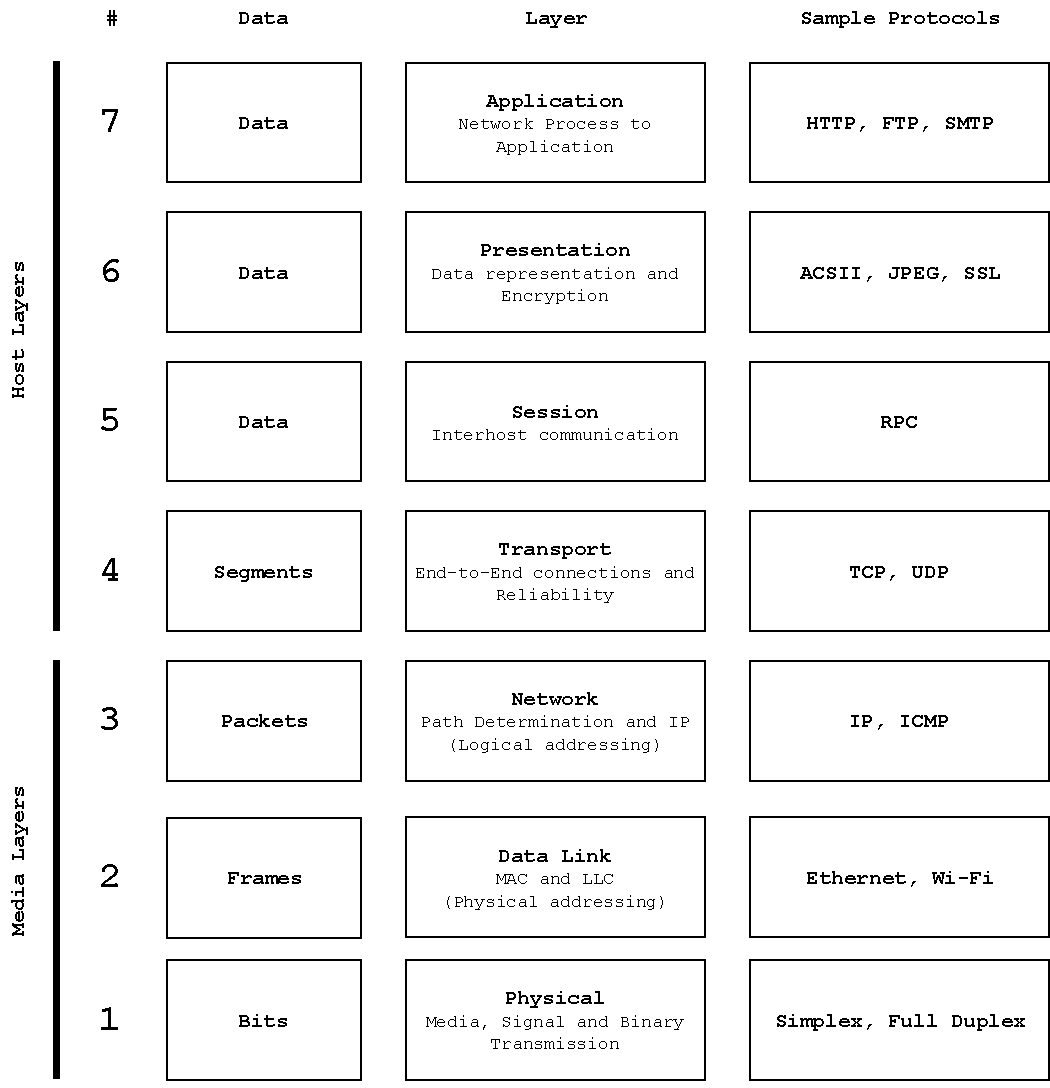
\includegraphics[width=.5\textwidth]{graphics/osi-modell.pdf}
\caption{OSI-Model (adapted from \citet{wiki:osi-model})}
\label{fig:osimodel}
\end{figure}

\subsection{Application Layer}
Incoming data\newline
Device applications like browsers, email clients, calenders,... are interacting only with this layer. The application layer provides an interface that comes from the underlying protocol like \gls{http} for Browser applications or \gls{smtp} for E-Mail applications. The data is in a consumable state and it is up to the application what to do with it.

Outgoing data\newline
Similar as for incoming data the application layer is also the entry point for device applications to send data using the protocol of the application layer like \gls{http}. 


\subsection{Presentation Layer}
Incoming data\newline
Preparing the data and making it consumable for the application layer is the task of the data layer. 
Hence, data has to be decrypted when it is encrypted, decompressed and put into the right format by decoding it.

Outgoing data\newline
Outing data can be encrypted, compressed and encoded by this layer.

\subsection{Session Layer}
Keeping the session and connection between two devices is one of the responsibilities of the session layer. It can also keep track of transmitted data so in case the connection is interrupted it can continue where it left off e.g. when a file transfer is interrupted the file does not be re-transmitted from the first byte. 

\subsection{Transport Layer}
Incoming segments\newline
The transport layer is responsible for reassembling incoming segments and putting them into the right order, for error handling e.g. deal with lost packets and to determine the optimal connection speed how to communicate with the other. 
The two main protocols are \gls{tcp} and \gls{udp}

Outgoing data\newline
Data that is sent is segmented into smaller chunks and further processed by the underlying protocol, e.g. \gls{tcp} adds a sequence number to each segment.

\subsection{Network Layer}
Incoming packets\newline
Incoming Packets are routed towards the receiver when the device is not the receiver and the receiver is not in the same network. Otherwise packets are  reassembled into segments and handed over to the transport layer.

Outgoing segments\newline
For outgoing segments the network layer is responsible for creating packets and routing them towards its destination.
The well known \gls{ip} is operating on this level. Segments provided by transport layer  are segmented into packets. Each packet gets a \gls{ip} packet header that contains the address of the sender, the adress of the receiver, a \gls{ttl}, the protocol with its version and other fields \cite{rfc791-ip}. The packets are then routed via routers towards the destination when the receiver address exists somewhere.

\subsection{Data Link Layer}
Incoming frames\newline
Tasks of this layer involve segmenting packets into frames and transmitting them within the same network.
Common networking components that are operating on this level are switches, hubs and network interface cards \cite{simoneau2006}.

Outgoing packets\newline
Packets received from the network layer are segmented into frames 

\subsection{Physical Layer}
The physical layer is the layer where the actual transport happens on a physical connection in form of electrical or optical signals.
Outgoing frames are transformed into bits (0,1) which can be represented as a signal.
Incoming bits are reassembled into frames and handed over to the data link layer.


\section{Overlay Network}
\begin{figure}[htb!]
\centering
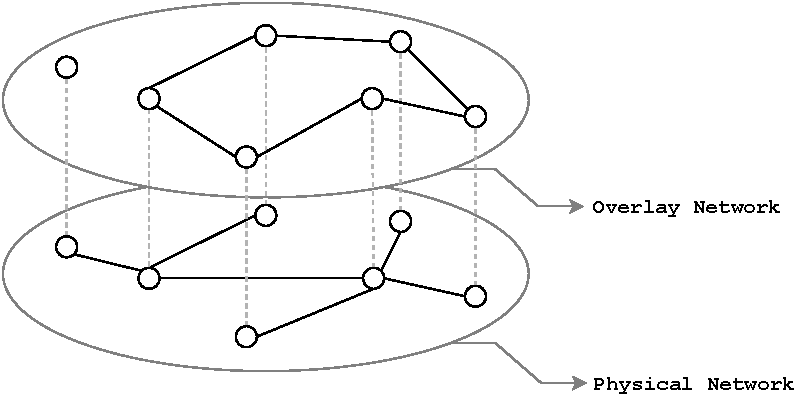
\includegraphics[width=.5\textwidth]{graphics/physical-vs-overlay-network.pdf}
\caption{Physical and overlay network example}
\label{fig:overlay}
\end{figure}
An overlay network is constructed on the application layer so is independent from the underlying physical network. 
Hence, devices that are connected with each other form the physical network, while the overlay network is constructed on top of it. The overlay network only cares about who is part of the network and not how the partner is reachable. 
While the physical communication has physical links between devices, the overlay network makes usage of virtual edges to connect devices that are not physically connected with each other. When a device wants to connect to a device that is not physically connected the overlay network can use indirect connections. That means when \textit{A} is connected to \textit{B} and \textit{B} is connected to \textit{C}, the overlay network allows \textit{A} to send data to \textit{C} via \textit{B}.
\cref{fig:overlay} shows a sample physical network and its derived sample overlay network.

As the underlying physical is transparent to the developer, the overlay network offers a huge design flexibility. The developer is free to chose her own network topology and protocol to use e.g. \gls{tcp} or \gls{udp}. However, the developer is responsible to maintain the virtual edges. This means when a device leaves the network, the overlay network has to be updated accordingly e.g. establish a replacement edge.

\section{Overlay Network Topologies}
The most common overlay network topologies are shown in \cref{fig:overlay-topologies}. In a centralised topology all devices are connected to one central device. A typical centralised example is the internet. The central device is a server and all other devices exchange information with that device. Advantages of this topology that it is easily manageable and the maintainer has full control over it. Thus, the provided information is always up to date and the maintainer can control who has access to it. However, a centralised network can not grow endlessly but only as big as the central device can handle the traffic. There is also a single point of failure. When the central device is not available anymore the whole network is offline.

\begin{figure}[htb!]
  \centering
    \subfloat[Centralised]{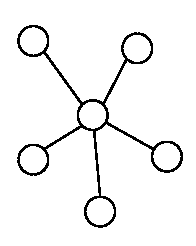
\includegraphics[width=0.25\textwidth]{graphics/overlay-network-centralised.pdf} \label{fig:overlay-topologies-a}}
    \subfloat[Hierarchical]{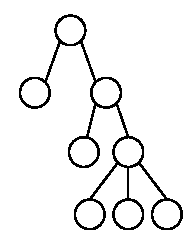
\includegraphics[width=0.25\textwidth]{graphics/overlay-network-hierarchical.pdf} \label{fig:overlay-topologies-b}}
	\subfloat[Decentralised]{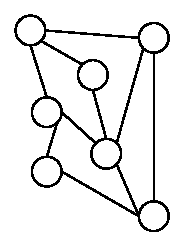
\includegraphics[width=0.25\textwidth]{graphics/overlay-network-decentralised.pdf} \label{fig:overlay-topologies-c}}
	\caption{Common overlay network topologies}
\label{fig:overlay-topologies}
\end{figure}

Are more scale-able and robust approach is a hierarchical overlay topology (\cref{fig:overlay-topologies-b}). The root node is still a single point of failure but when a node below crashes it does not affect the whole network anymore but only nodes underneath. By implementing load balancing techniques a hierarchical network also scales better because the workload can be distributed among child nodes.

To get rid of the single point of failure a decentralised overlay topology has to be used (\cref{fig:overlay-topologies-b}). In contrast to the previous mentioned topologies the decentralised one is completely unstructured and anyone can join in anywhere. Also nodes can connect to any other node in the network. However, as any node can be connected with another the network is hard to manage. The process of peers joining and leaving the network is called \textit{Churn} \cite[\S1]{stutzbach_rejaie_2006} and is a challenging part of decentralised networks.

In order to manage a decentralised network a common strategy is to build a mesh network.
